\documentclass{article}
\usepackage{array}
\newcolumntype{L}{>{\centering\arraybackslash}m{4cm}}
\usepackage[czech]{babel}
\usepackage[utf8]{inputenc}
\usepackage[unicode]{hyperref}
\usepackage{graphicx}
\usepackage{textcomp}
\usepackage[T1]{fontenc}
\usepackage[left=2cm, text={17cm, 24cm}, top=2cm]{geometry}
\usepackage[table,xcdraw]{xcolor}
\usepackage{caption}
\usepackage{color}
\usepackage{hyperref}
\hypersetup{
    colorlinks=true, % make the links colored
    linkcolor=blue, % color TOC links in blue
    urlcolor=red, % color URLs in red
    linktoc=all % 'all' will create links for everything in the TOC
}

\begin{document}

%%%%%%%%%%%%%%%%%TITULKA%%%%%%%%%%%%%%%%%% 

	\begin{titlepage}
		\begin{center}
			\textsc{\Huge Vysoké Učení Technické v Brně} \\[0.7cm]
			{\Huge Fakulta informačních technologií}
			\center
\includegraphics[width=0.5\linewidth]{./logo.png}

			\vspace{5cm}

			\textbf{{\Huge Dokumentace k projektu IFJ}}\\[0.4cm]
			\textbf{{\LARGE Implementace překladače imperativního jazyka IFJ19}}\\[0.4cm]
			\LARGE{Tým 072, varianta II}\\
			
		\end{center}
		\vfill

		\begin{flushleft}
			\begin{Large}
				\textbf{Šimon Sedláček}\hspace{10px}\textbf{(xsedla1h)}\hspace{10px}\textbf{25\% }\\[0.25cm]
				Marek Žiška\hspace{44px}(xziska03)\hspace{22px}25\%  \\[0.25cm]
				Martin Osvald\hspace{32px}(xosval03)\hspace{20px}25\% \\[0.25cm]
				Marek Sarvaš\hspace{37px}(xsarva00)\hspace{19px}25\% 
			\hfill
			Brno, 11.12.2019
			\end{Large}
		\end{flushleft}

	\end{titlepage}
%%%%%%%%%%%%%%%%%TITULKA%%%%%%%%%%%%%%%%%% 

%%%%%%%%%%%%%%%%%OBSAH%%%%%%%%%%%%%%%%%% 

	\tableofcontents
	\newpage
%%%%%%%%%%%%%%%%%OBSAH%%%%%%%%%%%%%%%%%% 


	\section{Úvod}
	\large{Tento dokument popisuje návrh a implementáciu prekladača imperatívneho jazyka IFJ19, čo je zjednodušená podmnožina jazyka Python 3. Cieľovým jazykom je trojadresný medzikód IFJcode19. 
	
	Prekladač je implementovaný ako konzolová aplikácia, čiže načíta vstup z štadardného vstupu, chybové hlášky sa vypisujú na štandarný chybový výstup a vygenerovaný medzikód IFJcode19 na štandardný výstup.}
	\newpage
	\section{Lexikkální analýza}
	Lexikálna analýza je implementovaná v module scanner.c. Úlohou lexikálnej analýzy je rozpoznávanie validných alebo chybných lexémov (tokenov) v prekladanom zdrojovom súbore. Postupne ako syntaktická analýza vyhodnocuje LL pravidlá, tak zároveň volá lexikálnu analýzu o nasledujúce tokeny, teda poskytuje rozhranie pre syntaktickú analýzu formou funkcie get\_token().
	Lexikálna analýza vždy vracia jeden aktuálny a validný token. Správnosť tokenu sa určuje pomocou konečného automatu, ktorý je popísaný nižšie formou diagramu.

	\section{Syntaktická analýza}
	Ústrednou časťou prekladača je syntaktický analyzátor, ktorý má jadro v module parser.c. V tomto module sa nachádza implementácia pravidiel pre rekurzívny zostup, volá sa tu precedenčná syntaktická analýza, funkcie pre generovanie častí kódu, sémantické akcie. Druhou časťou  syntaktického analyzátoru je potom modul precedence\_analysis.c, ktorý má na starosť syntaktickú analýzu výrazov.
	
	Syntaktický analyzátor využíva funkciu get\_token() poskytovanú lexikálnym analyzátorom a implementuje nad ňou abstraktnejšiu operáciu next\_token() s ošetrením chybových stavov a prípadným načítáním uloženého tokenu z odkladiska.
	
	Súčásťou syntaktického analyzátoru je globálna štruktúra parser\_data, ktorá okrem inštancií lokálnych a globálnych tabuliek symbolov obsahuje premennú curr\_token uchovávajúcu  aktuálny token, odkladisko tokenov token\_stash, ukazatele na symboly, aktuálne definované a aktuálne volané funkcie, indikátor in\_function, ktorý obsahuje informaciu o tom, či sa nachádzame vo vnútri definície funkcie a indikátor psa\_state. Psa\_state obsahuje informáciu pre PSA,ktorá jej umožňuje podľa kontextu spracovávaného výrazu vykonávať sémantické akcie a generovať kód pre príslušné konštrukcie. Ako ďalšie táto štruktúra obsahuje premenu undef\_symbol, ktorá umožňuje vykonávať niektoré sémantické kontroly týkajúce sa tieňovania globálnych premenných a obecné definície premenných.
	
	Syntaktickú analýzu hlavného tela programu sme založili na LL(1) gramatike. Pravidlá implementované v module parser.c reflektujú nami vytvorenú LL gramatiku s výnimkou dvoch prípadov:
	Pravidlá pre neterminály <term> a <literal> neboli vo výslednej implementácii syntaktického analyzátoru využité - vo výslednej implementácii sa ukázali ako zbytočné a bolo prehľadnejšie tieto pravidla implementovat priamo v rámci iných pravidiel.
	Pre pravidlá <value> a <rest> bolo nutné nájsť spôsob ako odlíšiť začiatok aritmetického výrazu od volania funkcie. Z tohto dôvodu sme implementovali jednoduchú štruktúru token\_stash, ktorá nám umožňuje odložiť na stranu aktuálne zpracovávaný token a pozrieť sa až o dva tokeny dopredu. Vďaka tomuto nahliadnutiu je pak syntaktický analyzátor schopný rozhodnúť, či se bude jednať o výraz (pričom v tomto prípade je predané riadenie PSA) alebo volanie funkcie.
	

	\subsection{Precedenčná syntaktická analýza}
	Precedenčná syntaktická analýza je implementovaná v súbore precedence\_analysis.c. Túto analýzu volá syntaktický analyzátor rovnakým spôsobom ako iné pravidlá z LL gramatiky, ak narazí na výraz. 
	Spracovávaný výraz sa vyhodnocuje pomocou precedenčnej tabuľky a pravidiel. V tabuľke je skrátený zápis relačných operátorov(riadok a stĺpec označený “r”), pretože majú rovnakú asociativitu a prioritu. Takýmto spôsobom sú relačné operátory spracované aj vo výslednom programe, kde sú navyše takto skrátene aj operátory “+”,”-” a “*”,”/”,”//”. Na vyhodnocovanie výrazu je použitý zásobník, na ktorého začiatok sa vloží “¨\$”. Pomocou prvého terminálu na zásobníku a novo načítaného tokenu sa získa operácia z tabuľky( vloženie na zásobník, redukcia alebo koniec analýzy). Pri redukcii sa aplikuje  pravidlo, ktoré odstráni dané terminály zo zásobníku a pridá neterminál na jeho vrchol. Analýza končí pri absencii pravidla počas operácie redukcie. Každý novo načítaný token sa ukladá do poľa v infixovej notácii kvôli nasledujúcej sémantickej analýze daného výrazu, ktorá sa volá až po úspešnom dokončení syntaktickej precedenčnej analýzy.
	

	\section{Sémantická analýza}
	Sémantické akcie využívané v rámci rekurzívneho zostupu a z časti aj PSA sú implementované v module semantic.c. 
	Okrem štandardných sémantických kontrôl týkajúcích sa štandartných prípadov definícií premenných a funkcií sme pri implementácií narazili na dva zložitejšie prípady sémantických akcií.
	\subsection{Referencia lokálnej promennej pred jej definíciou}
	Jedným z týchto prípadov je referencia globálnej premennej vo funkcii a následná definícia lokálnej premennej s rovnakým menom. Pre odhalenie tohto prípadu sa pri využití globálnej premennej vo funkcii uloží do lokálnej tabuľky symbolov nová nedefinovaná lokálna premenná. Ak by sa užívateľ pokúsil následne definovať túto lokálnu premennú, sémantická analýza ukončí preklad s chybou 3.
	\subsection{Kontrola dependencií funkcií a lineárny zoznam symbolov}
	Kvôli kontrole dependencií funkcií pri vzájomných volaniach, je pri volaní funkcie z hlavného tela programu nutné prejsť rekurzívne zoznamy dependencií všetkých dependencií volanej funkcie. Ak sú všetky dependencie definované, potom je volanie funkcie v poriadku. Tu však nastal problém s možnosťou nekonečnej rekurzie, ak by se dve alebo viacero funkcií volalo kruhovo navzájom.
	Tento problém sme riešili pomocou lineárneho zoznamu už skontrolovaných funkcií - ak sa symbol kontrolovanej funkcie už nachádza v tomto zozname, nie je nutné kontrolovať ďalej jeho dependencie.
	
	\subsection{Precedenčná sémantická analýza}
	Precedenčná sémantická analýza je volaná po úspešnom skončení precedenčnej syntaktickej analýzy, ktorá jej predáva pole token-ov v infixovej notácii. Ako prvá sa prevedie kontrola deklarácie všetkých premenných vo výraze, ak sa nájde nedefinovaná premenná sémantická analýza končí chybou. Po kontrole definícií premenných sa prevedie konverzia infixovej notácie na postfixovú. Následne sa postfixový zápis vyhodnocuje. Všetky operátory sú binárneho typu preto sa vždy vyhodnocujú dva operandy a operátor. Táto dvojica operandov je sémanticky kontrolovaná na správne typy vzhľadom na  daný operátor prípadne delenie nulou pri celočíselnom delení. Po úspešnom ukončení sémantickej analýzy sa podľa hodnoty psa\_state volá generovanie kódu, ktorému sa ako parametre predáva aktuálna dvojica operandov a operátor. Úspešné vygenerovanie trojadresného kódu vráti názov premennej medzi-výsledku, ktorá sa ako token uloží na zásobník vyhodnocovania postfixu pre ďalšie spracovanie.
	\section{Generovanie cieľového kódu}
	V priebehu syntaktickej a sémantickej analýzy sú v rámci rekurzívneho zostupu a PSA volané funkcie pre generovanie výsledného kódu. Cieľový kód je uchovávaný v štruktúre s názvom generate\_strings\_output\_t. Táto štruktúra obsahuje päť dynamických stringov, ktoré sa volajú : main, function\_definitions, errors, stash, print. Do týchto stringov sa ukladá cieľový kód jazyka. 
	Na začiatku generovania sa alokujú dynamické stringy.  Do stringu function\_definitions sa pridávajú vstavané funkcie jazyka IFJ19. Do stringu errors sa pridajú chybové náveští s návratovými kódmi. 
	\subsection{Generovanie definície premenných}
	Keď sme riešili problém definícií premenných v cykloch while a if-else, tak sme prišli s riešením s pomocí stringu stash. Definície premenných se vždy generujú do stringu main alebo \\function\_definitions v závislosti na tom, či sa aktuálne nachádzame v globálnom alebo v  lokálnom kontexte. Ostatné príkazy a konštrukcie sa generujú do stringu stash. Pri opustení aktuálneho kontextu (lokálneho či globálneho) sa string stash pripojí na koniec stringu main alebo function\_definitions.
	\subsection{Generovanie unikátnych názvov premenných, náveští}
	Na generovanie názvov náveští a premenných využívame štruktúru unique\_id\_t. Táto štruktúra má deväť int-ových atribútov, ktoré slúžia ako počítadlá na vytvorenie identifikátorov. Tieto atribúty potom používame ako parametre do funkcie create\_unique\_variable, ktorá nám vytvorí unikátny názov. Podľa potreby potom jednotlivé atribúty z unique\_id\_t iterujeme, aby sa nám zachovala unikátnosť.
	\subsection{Generovanie výrazu}
	Každý výraz je behom syntaktickej analýzy ukladaný do dátového zásobníku . V rámci postfixu je tento výraz spracovávaný a popritom je volaná funkcia generate\_expression. Táto funkcia prijíma vždy dva operandy a jeden operátor, a na základe daného operátoru prepína medzi tým aký kód sa vygeneruje pre daný výraz. Pri generovaní voláme pomocné funkcie ako  check\_if\_op\_type\_eq, generate\_jumpeq\_string\_string, convert\_ints\_to\_floats, \\append\_token\_variable\_to\_assembly, append\_token\_operands\_to\_assembly, ktoré nám \\pomáhajú uľahčiť kód a jeho sprehľadnenie.
	
	\section{Datové struktury a použité algoritmy}
	\subsection{Tabuľka symbolov}
	Súčasťou zadania zo strany predmetu IAL bol požiadavok na implementáciu tabulky symbolov. V našom prípade sa jednalo o druhú variantu zadania - tabulka symbolov mala být implementována ako tabulka s rozptýlenými položkami.
	
	Tabuľku symbolov sme teda implementovali jako TRP s explicitním zreťazením. Ako rozptyľovaciu funkciu sme použili variantu funkce PJW, GNU Hash ELF. Veľkosť pole bucketov v tabuľke sme zvolili na 27457 položek. Pre takto vysokú hodnotu bolo nepravdepodobné, že by naplnenie tabulky presiahlo 75\% a začalo by dochádzať ku kolíziam a to ani v prípade väčších vstupných programov.
	
	Položkou v tabuľke symbolov je potom štruktúra symbol, ktorá má okrem ukazovateľa na ďalší prvok v zozname a svojho identifikátoru ešte atribúty type  (určuje typ symbolu -funkcia, premenná) a attributes (únia uchovávajúca atribúty špecifické pre daný typ symbolu). Pre premennú má únia attributes len položku defined, ktorá je využívaná pri sémantických kontrolách. Pre funkciu má únia attributes ešte položky param\_count (počet parametrov potrebných pre volanie funkcie).
	
	Ďalej dvojicu  špeciálnych atribútov, ktoré sa využívajú pri sémantických kontrolách dependencií funkcií pri vzájomných volaniach. Jedná sa o atribút depends - dynamické pole ukazovateľov na symboly iných funkcií; a atribút dep\_len, ktorý drží informáciu o aktuálnej veľkosti poľa dependencií.
	
	\subsection{Nekonečný string}
	Pretože bolo nutné mať v rámci lexikálnej analýzy možnosť načítať ľubovoľne dlhé lexémy, implementovali sme si vlastnú dynamickú štruktúru string, ktorá nám prácu s potenciálne nekonečnými reťazcami umožňuje. Táto štruktúra taktiež našla využitie v rámci generovania kódu, kde slúži ako vyrovnávacia pamäť a umožňuje flexibilnejšiu manipuláciu s vygenerovaným kódom.
	\subsection{Obecný stack}
	Pri implementaci sme v rámci lexikálnej analýzy, PSA i generovania kódu pre niektoré operácie potrebovali využít strukturu stack. Prípady využitia stacku sa však lišily natoľko, že sme ako najlepšie riešenie vyhodnotili implementaciu obecného stacku založeného na jednosmernom viazanom zozname, ktorý môže uchovávat data obecného typu.
	
	\section{Tímová práca}
	V rámci tímovej spolupráce sme využívali verzovací systém Git. Pre komunikáciu sme zvolili službu Discord.
	Zo začiatku sme mali problém projekt obsiahnuť - dlho nám trvalo, kým sme sa ako tím získali jasný prehľad o tom, akým smerom sa má projekt uberať. Napriek tomu sa nám nakoniec projekt podaril včas a dúfame v štastný koniec.
	
		Prácu na projekte sme medzi členov tímu rozdelili nasledovne:
	\begin{center}
		\begin{tabular}{| L | L}
			\hline
			\textbf{Šimon Sedláček (xsedla1h)} & \multicolumn{1}{m{12cm}|}{tabuľka symbolov, syntaktická analýza, sémantická analýza, dynamický string, testovanie }\\\hline
			Marek Sarvaš (xsarva00) & \multicolumn{1}{m{12cm}|}{precedenčná syntaktická a sémantická analýza, testovanie, dokumentácia }\\\hline
			Marek Žiška (xziska03) & \multicolumn{1}{m{12cm}|}{lexikálna analýza, generovanie kódu, testovanie, dokumentácia}\\\hline
			Martin Osvald (xosval03) & \multicolumn{1}{m{12cm}|}{generovanie kódu, obecný stack, dynamický string , testovanie, dokumentácia }\\\hline
		\end{tabular}
	\end{center}
	
	
	
	
	\section{Diagram konečného automatu použitého v lexikálnom analyzátore }
	\center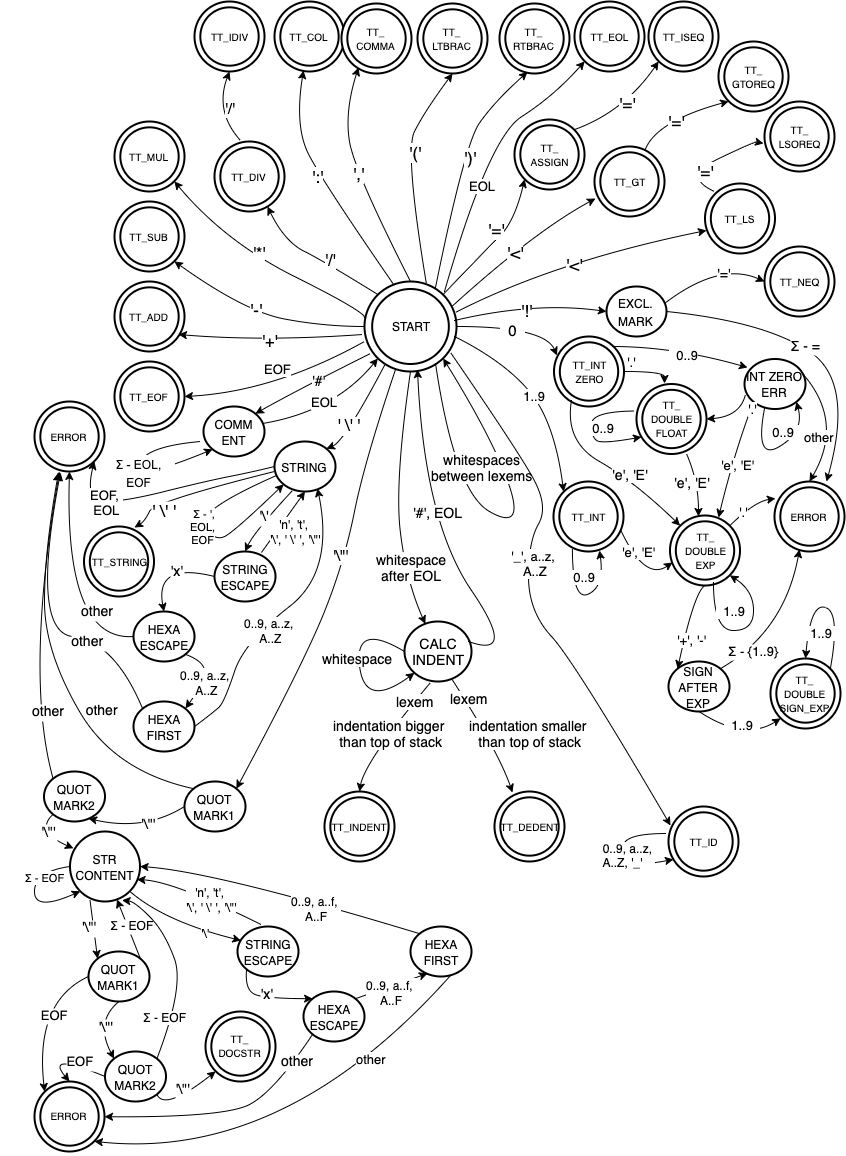
\includegraphics[width=0.9\linewidth]{./with_error_state.png}
	\section{LL gramatika}
	\center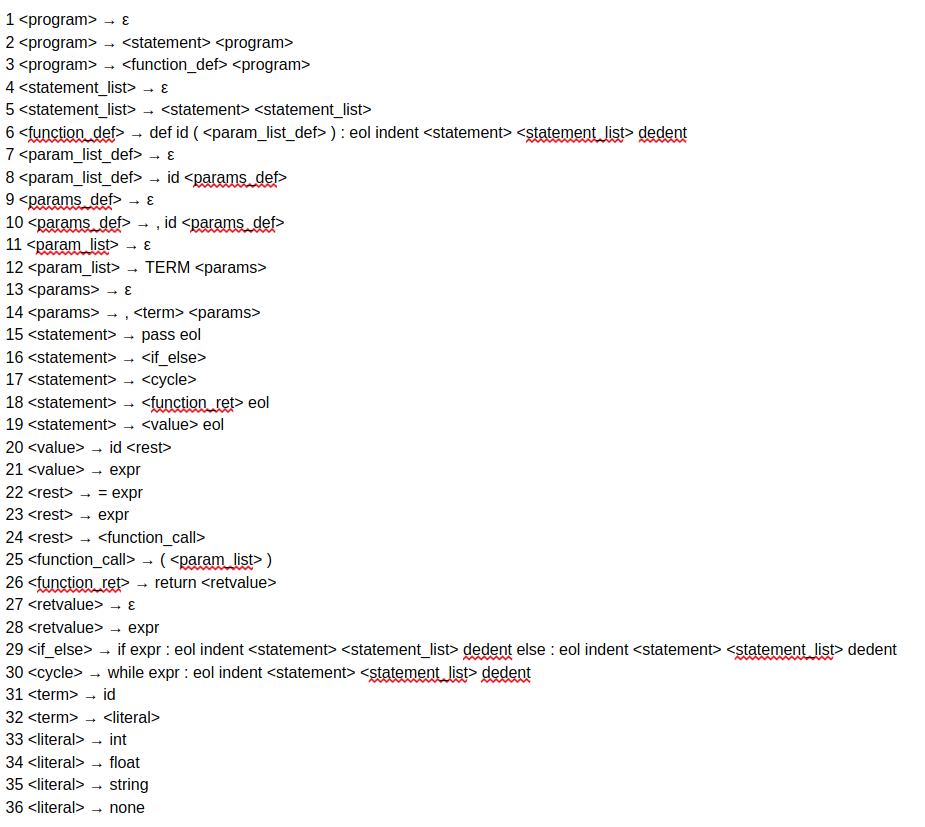
\includegraphics[width=0.9\linewidth]{./LLgrammar.png}
	\section{LL tabuľka }
	\center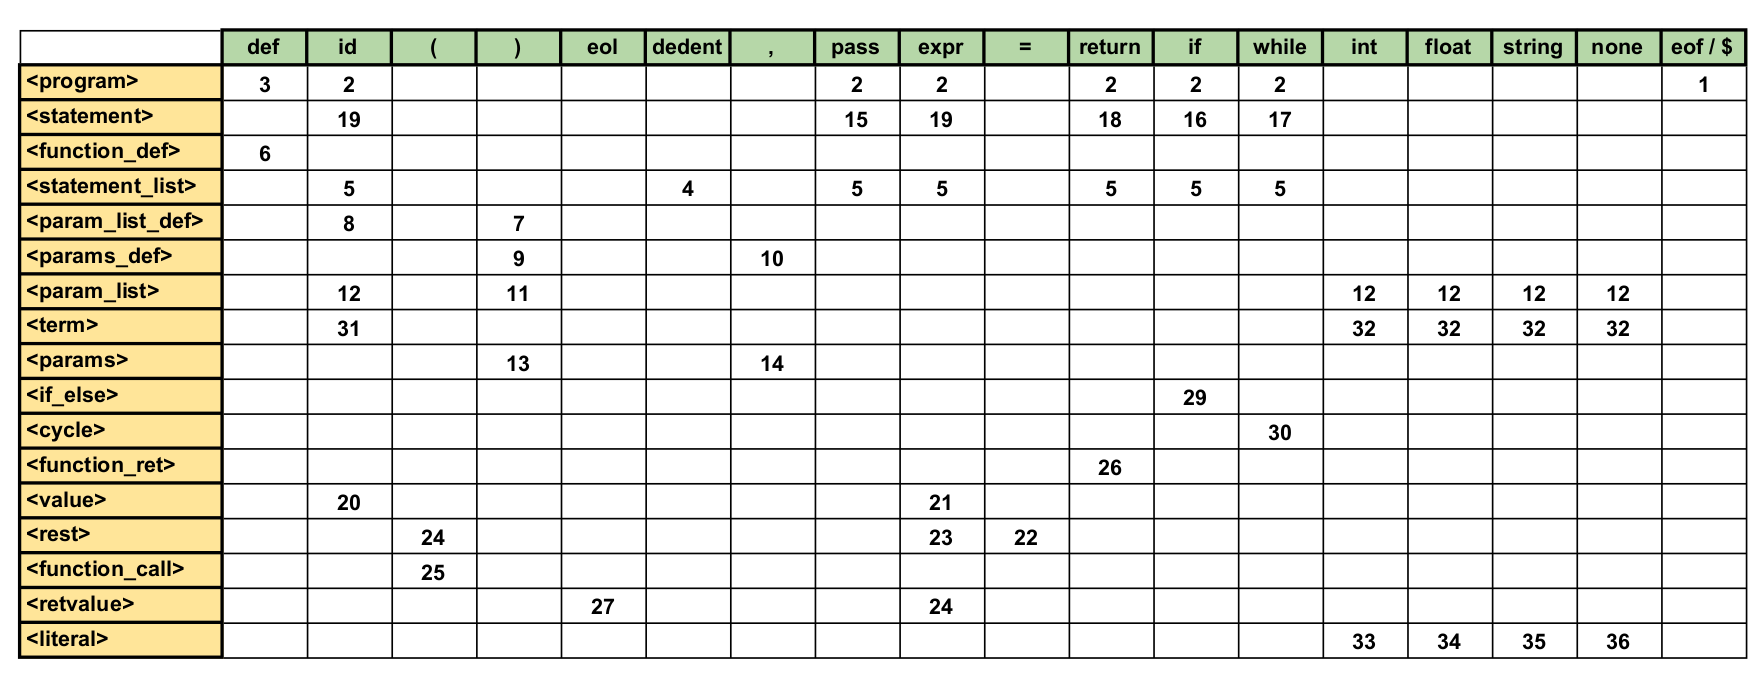
\includegraphics[width=1\linewidth]{./LLtable.png}
	\section{Tabuľka popisujúca precedenčnú analýzu }
	\center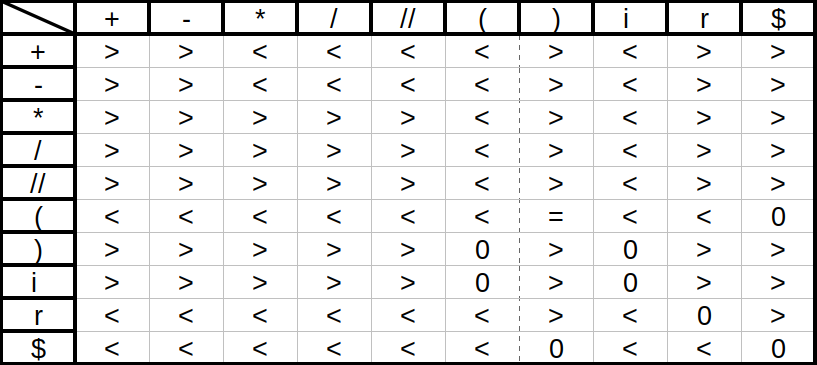
\includegraphics[width=1\linewidth]{./precedence_table.png}
	
\end{document}
